\documentclass[pdflatex,compress,mathserif]{beamer}

%\usetheme[dark,framenumber,totalframenumber]{ElektroITK}
\usetheme[darktitle,framenumber,totalframenumber]{ElektroITK}

\usepackage[utf8]{inputenc}
\usepackage[T1]{fontenc}
\usepackage{lmodern}
\usepackage[bahasai]{babel}
\usepackage{amsmath}
\usepackage{amsfonts}
\usepackage{amssymb}
\usepackage{graphicx}
\usepackage{multicol}

\newcommand*{\Scale}[2][4]{\scalebox{#1}{$#2$}}%

\title{Pengolahan Sinyal Digital}
\subtitle{Transformasi Z}

\author{Tim Dosen Pengampu}

\begin{document}

\maketitle

\begin{frame}
	\frametitle{Transformasi Fourier}
	\begin{itemize}
		\item T. Fourier:
		\[ X(e^{j \omega}) = \sum_{n = -\infty}^{+ \infty} x(n) e^{-j\omega n} \]
	\end{itemize}
\end{frame}

\begin{frame}{Transformasi Fourier}
	\begin{itemize}
		\item Syarat konvergensi:
		\begin{align*}
		| X(e^{j \omega}) | &= \left| \sum_{n = -\infty}^{+ \infty} x(n) e^{-j\omega n} \right| \leq \sum_{n = -\infty}^{+ \infty} | x(n) | | e^{-j\omega n} | \\
		| X(e^{j \omega}) | &\leq \sum_{n = -\infty}^{+ \infty} | x(n) | | e^{-j\omega n} | \\
		&\leq \sum_{n = -\infty}^{+ \infty} | x(n) |
		\end{align*}
		\item Sehingga $ X(e^{j \omega}) $ konvergen jika $ \sum\limits_{n = -\infty}^{n = +\infty} | x(n) |< \infty $ (\textit{summable})
		\item Sistem stabil $\Leftrightarrow$ $ H(e^{j \omega}) $ konvergen
	\end{itemize}
\end{frame}

\begin{frame}
	\begin{enumerate}
		\item $ x(n) = (\frac{1}{2})^n u(n) $; $ \sum\limits_{-\infty}^{+\infty} |x(n)| = 2 $ $\rightarrow$ T. Fourier konvergen
		\item $ x(n) = (2)^n u(n) $; $ \sum\limits_{-\infty}^{+\infty} |x(n)| = \infty $ $\rightarrow$ T. Fourier divergen
	\end{enumerate}
\end{frame}

\begin{frame}
	\begin{itemize}
		\item Solusinya adalah $ x(n) $ dikali dengan eksponensial $ r^{-n} $
	\end{itemize}
	\begin{align*}
		X_r(e^{j \omega}) &= \sum\limits_{n = -\infty}^{+\infty} [ x(n) r^{-n} ]e^{-j \omega n} \\
		&= \sum\limits_{n = -\infty}^{+\infty} x(n)(re^{j \omega })^{-n} \\
		&= \sum\limits_{n = -\infty}^{+\infty} x(n)(z)^{-n}
	\end{align*}
\end{frame}

\begin{frame}
	\frametitle{Transformasi Z}
	\begin{itemize}
		\item[] \[ z = re^{j\omega} \]
		\item[] \[ X(z) = \sum_{n = -\infty}^{+\infty} x(n)z^{-n} \]
		\item[] \[ X(e^{j\omega}) = X(z)\left|_{z = e^{j \omega}}\right. \]
		\item[] Konvergen jika
		\[ \sum\limits_{n = -\infty}^{+\infty} |x(n)r^{-n}| < \infty \]
	\end{itemize}
\end{frame}

\begin{frame}
	\begin{align*}
		x(n) &= \left(\frac{1}{2}\right)^n u(n) \\
		X(z) &= \sum\limits_{n=0}^{\infty} \left(\frac{1}{2}\right)^n z^{-n} = \sum\limits_{n=0}^{\infty} \left(\frac{1}{2} z^{-1}\right)^n \leftarrow \text{\textit{deret geometri}}\\
		&= \frac{1}{1 - \frac{1}{2}z^{-1}} = \frac{z}{z - \frac{1}{2}}
	\end{align*}
	konvergen jika
	\begin{align*}
		\sum_{0}^{\infty} \left| \left(\frac{1}{2} z^{-1}\right)^n \right| < \infty &\text{;} \text{ agar finite maka }\left| \left(\frac{1}{2} z^{-1}\right) \right| < 1 \\
		\sum_{0}^{\infty} \left| \left(\frac{1}{2} z^{-1}\right)^n \right| < \infty&\implies |z| > \frac{1}{2}
	\end{align*}
\end{frame}

\begin{frame}
	\frametitle{Region of Convergence}
	\begin{itemize}
		\item T. Fourier konvergen jika konvergensi T. Z termasuk didalamnya $ |z| = 1 $. Apakah sudah terpenuhi?
		\item Ada tidaknya T. Fourier dalam bentuk ROC (region of convergence) dari T. Z.
	\end{itemize}
	\begin{center}
		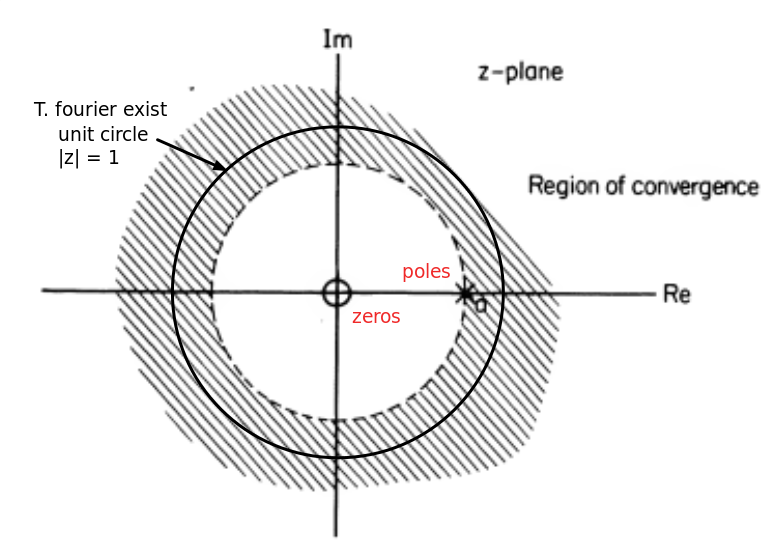
\includegraphics[width=0.7\linewidth]{img/img01}
	\end{center}
\end{frame}

\begin{frame}
	\begin{align*}
		x(n) &= -\left(\frac{1}{2}\right)r(-n-1) \\
		X(z) &= \frac{1}{1-\frac{1}{2}z^{-1}} = \frac{z}{z - \frac{1}{2}}
	\end{align*}
	konvergen jika
	\begin{align*}
	\sum_{-1}^{-\infty} \left| \left(\frac{1}{2} z^{-1}\right)^n \right| < \infty &\text{;} \text{ agar finite maka }\left| \left(\frac{1}{2} z^{-1}\right) \right| > 1 \\
	\sum_{-1}^{-\infty} \left| \left(\frac{1}{2} z^{-1}\right)^n \right| < \infty&\implies |z| < \frac{1}{2}
	\end{align*}
\end{frame}

\begin{frame}
	\begin{center}
		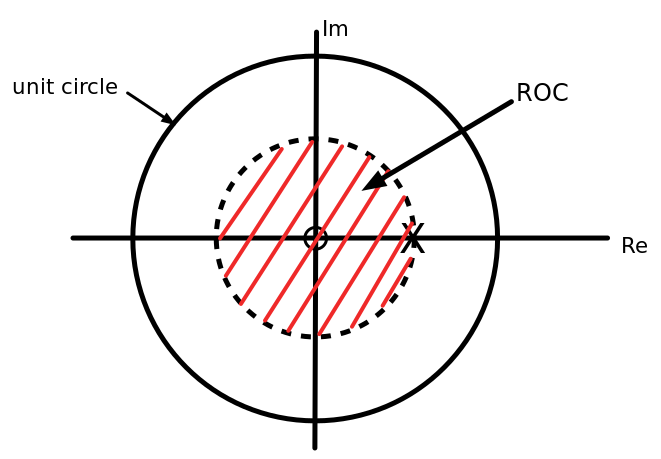
\includegraphics[width=0.5\linewidth]{img/img02}
	\end{center}
	\begin{itemize}
		\item Jika dibandingkan dengan contoh sebelumnya, hasil T.Z nya sama tapi ROC nya berbeda.
		\item Sehingga penting menampilkan ROC.
		\item T.Z $\rightarrow$ hasil T.Z. dan ROC
	\end{itemize}
\end{frame}

\begin{frame}
	\frametitle{Region of Convergence Properties}
	\begin{enumerate}
		\item Tidak ada poles di dalam ROC
		\item Region of Convergence dibatasi oleh poles or (zeros / $\infty$)
		\item Finite length sequences \[ 0 < |z| < \infty\]
		\item Right-sided sequences: $ x(n) = 0; \quad n < \text{ some value} $, \[ R_{x-} < |z| < \infty \] $ R_{x-} $: poles paling luar
	\end{enumerate}
\end{frame}

\begin{frame}
	\begin{enumerate}
		\setcounter{enumi}{4}
		\item Left-sided sequences: $ x(n) = 0; \quad n>\text{ some value} $, \[ 0< |z| < r_{x+} \] $ R_{x+} $: poles paling dalam
		\item Two-sided sequences: \[ R_{x-} < |z| < R_{x+} \]
	\end{enumerate}
\end{frame}

\begin{frame}
	\begin{center}
		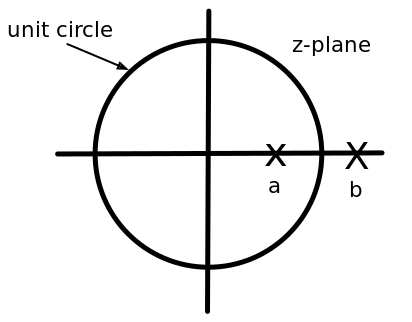
\includegraphics[width=0.5\linewidth]{img/img03}
	\end{center}
	\[ 
		\begin{matrix}
		\text{ROC} & \text{sisi yang mana?} & \text{T. Fourier?} \\
		|z| < a & \text{left-sided} & \text{tidak ada}\\
		a < |z| < b & \text{two-sided} & \text{ada}\\
		|z| > b & \text{right-sided} & \text{tidak ada}\\
		\end{matrix}
	\]
\end{frame}

\begin{frame}
	\begin{itemize}
		\item Konvolusi sequence = perkalian T. Z dari sequence-nya
		\begin{align*}
			y(n) &= x(n) * h(n) \\
			Y(z) &= X(z)H(z)
		\end{align*}
		sama seperti T. Fourier
		\item T.Z dari unit sample response dari sistem sebagai system function
		\begin{align*}
			H(z) \triangleq \text{ system function}
		\end{align*}
		\item Stable $\rightarrow$ summable $\Leftrightarrow$ unit circle di dalam ROC
		\item Causal $ \implies $ $ h(n) $ right-sided $ \implies $ ROC di luar poles yang paling luar.
	\end{itemize}
\end{frame}

\begin{frame}
	Diketahui sistem dalam linear constant coefficient difference:
	\[ y(n) - \frac{1}{2} y(n-1) = x(n) \]
	sifat yang digunakan:
	\begin{align*}
		y(n) &\leftrightarrow Y(z) \\
		y(n+n_0) &\leftrightarrow z^{n_0}Y(z)
	\end{align*}
	\begin{align*}
		Y(z) - \frac{1}{2}z^{-1}Y(z) &= X(z) \\
		H(z) &= \frac{Y(z)}{X(Z)} = \frac{1}{1 - \frac{1}{2}z^{-1}} \leftarrow \text{ system function}
	\end{align*}
	Bagaimana dengan ROC?
\end{frame}

\begin{frame}
	\begin{multicols}{2}
		\begin{center}
			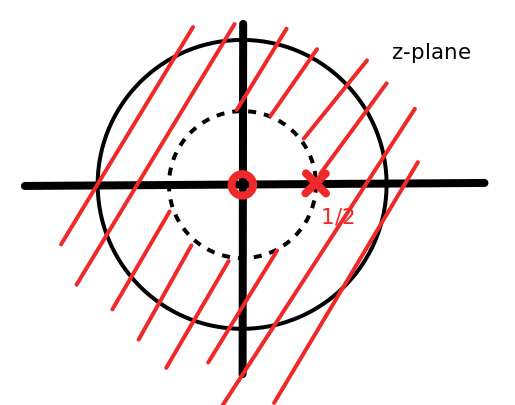
\includegraphics[width=\linewidth]{img/img04}
		\end{center}
	\columnbreak
	\begin{itemize}
		\item Perhatikan unit circle-nya. Punya T. Fourier? Ya $\rightarrow$ \textbf{Stable}
		\item Right-side $\rightarrow$ \textbf{Causal}
		\[ h(n) = \frac{1}{2}^n u(n) \]
	\end{itemize}
	\end{multicols}
\end{frame}

\begin{frame}
	\begin{multicols}{2}
		\begin{center}
			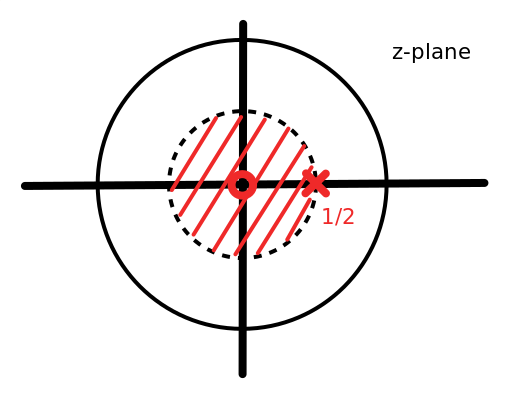
\includegraphics[width=\linewidth]{img/img05}
		\end{center}
		\columnbreak
		\begin{itemize}
			\item Perhatikan unit circle-nya. Punya T. Fourier? Tidak $\rightarrow$ \textbf{Not stable}
			\item Left sided $\rightarrow$ \textbf{Not causal}
			\[ h(n) = -\frac{1}{2}^n u(-n-1) \]
		\end{itemize}
	\end{multicols}
\end{frame}

\begin{frame}
	\frametitle{Kesimpulan}
	\begin{enumerate}
		\item Transformasi Z ada untuk mengatasi permasalahan konvergensi dalam Transformasi Fourier.
		\item Transformasi Z dari sequence adalah eksponensial berupa rasio dari polinomial yang kemudian dapat dijelaskan dalam poles dan zeros.
		\item Tidak hanya poles dan zeros, harus dijelaskan Region of Convergence (ROC) dari Transformasi Z-nya. Karena hasil Transformasi Z bisa sama tapi Region of Convergence-nya berbeda.
		\item Region of Convergence juga dapat menjelaskan left-sided, right-sided, atau two-sided dari sequence.
	\end{enumerate}
\end{frame}

\begin{frame}
	\frametitle{Latihan Soal 1}
	\begin{itemize}
		\item Apakah sequence berikut ini memiliki Transformasi Fourier yang konvergen?
		\begin{enumerate}
			\item $ x(n) = 2^n u(n) $
			\item $ x(n) = 2^n u(-n) $
		\end{enumerate}
	\end{itemize}
\end{frame}

\begin{frame}
	\frametitle{Jawaban Latihan Soal 1}
	\begin{itemize}
		\item Transformasi Fourier yang konvergen jika sequence harus benar-benar \textit{summable} atau \textit{square summmable} (dengan kata lain memiliki \textit{finite energy}). Maka
		\begin{enumerate}
			\item $ x(n) = 2^n u(n) \rightarrow $ \textbf{tidak konvergen}
			\item $ x(n) = 2^n u(-n) \rightarrow $ \textbf{konvergen}
		\end{enumerate}
	\end{itemize}
\end{frame}

\begin{frame}
	\frametitle{Latihan Soal 2}
	\begin{itemize}
		\item Untuk setiap sequence berikut ini, gambarlah pole-zero dan transformasi z nya. Tambahkan juga Region of Convergence-nya.
		\begin{enumerate}
			\item $ \delta(n) + \left( \frac{1}{2} \right)^n u(n) $
		\end{enumerate}
	\end{itemize}
\end{frame}

\begin{frame}
	\frametitle{Jawaban Latihan Soal 2}
	\begin{enumerate}
		\item $ x(n) = \delta(n) + \left( \frac{1}{2} \right)^n u(n) $
		\begin{align*}
			X(z) &= \sum_{n = -\infty}^{+\infty} x(n)z^{-n} \\
			&= \sum_{n = -\infty}^{+\infty} \delta(n) z^{-n} + \sum_{n = -\infty}^{+\infty} \left(\frac{1}{2}\right)^n u(n) z^{-n} \\
			&= 1 + \sum_{n=0}^{\infty} \left(\frac{1}{2}z^{-1}\right)^n \\
		\end{align*}
	\end{enumerate}
\end{frame}

\begin{frame}{Jawaban Latihan Soal 2}
	\begin{enumerate}
		\item[]
		\begin{align*}
		\sum_{n=0}^{\infty} \left(\frac{1}{2}z^{-1}\right)^n &= \frac{1}{1 - \frac{1}{2}z^{-1}} \quad \text{untuk } \left|\frac{1}{2}z^{-1}\right| < 1.
		\end{align*}
		\begin{align*}
		X(z) &= 1 + \frac{1}{1 - \frac{1}{2}z^{-1}} = \frac{2 - \frac{1}{2}z^{-1}}{1 - \frac{1}{2}z^{-1}};\quad |z| > \frac{1}{2}
		\end{align*}
	\end{enumerate}
\end{frame}

\begin{frame}{Jawaban Latihan Soal 2}
	\begin{center}
		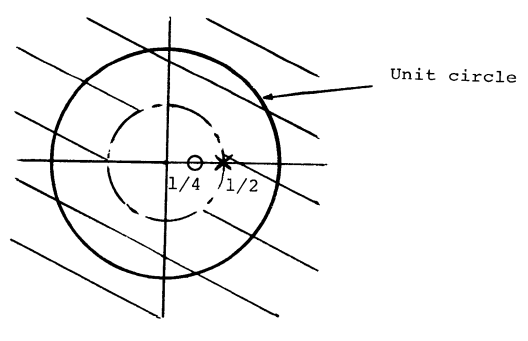
\includegraphics[width=0.7\linewidth]{img/img06}
	\end{center}
\end{frame}

\end{document}
